\documentclass[twoside, 11pt]{exam}

\usepackage[T1]{fontenc}
\usepackage[utf8]{inputenc}
\usepackage[dutch]{babel}

\usepackage[font={small,sf},labelfont={bf},labelsep=endash]{caption}
\usepackage{fouriernc}
\usepackage[detect-all, binary-units, separate-uncertainty=true,
            per-mode=symbol, retain-explicit-plus, range-phrase={ tot },
            list-final-separator={ en }, output-decimal-marker={,}]
            {siunitx}

\usepackage{setspace}
\setstretch{1.2}

\setlength{\parskip}{\smallskipamount}
\setlength{\parindent}{0pt}

\usepackage{geometry}
\geometry{a4paper, vmargin=3cm, inner=3cm, outer=2cm, head=14pt}

\usepackage{float}

\usepackage[fleqn]{amsmath}
\numberwithin{equation}{section}
\numberwithin{figure}{section}

\usepackage{graphicx}
\graphicspath{{Figures/}}
\usepackage{subfig}

\usepackage[svgnames]{xcolor}
\usepackage{tikz}
\usepackage{tikz-3dplot}
\usepackage{pgfplots}
\usetikzlibrary{plotmarks,circuits.ee.IEC,pgfplots.groupplots,external,calc}
\pgfplotsset{compat=1.3}

\usepackage{minted}
\usepackage{amsthm}
\usepackage{relsize}
\usepackage{xspace}
\usepackage{url}
\usepackage{sansmath}
\usepackage{titling}


\theoremstyle{plain}
\newtheorem*{note}{Note}


\newcommand{\figref}[1]{Figuur~\ref{#1}}

\newcommand{\hisparc}{\textsmaller{HiSPARC}\xspace}
\newcommand{\kascade}{\textsmaller{KASCADE}\xspace}
\newcommand{\sapphire}{\textsmaller{SAPPHiRE}\xspace}
\newcommand{\jsparc}{\textsmaller{jSparc}\xspace}
\newcommand{\hdf}{\textsmaller{HDF5}\xspace}
\newcommand{\aires}{\textsmaller{AIRES}\xspace}
\newcommand{\csv}{\textsmaller{CSV}\xspace}
\newcommand{\python}{\textsmaller{PYTHON}\xspace}
\newcommand{\corsika}{\textsmaller{CORSIKA}\xspace}
\newcommand{\labview}{\textsmaller{LabVIEW}\xspace}
\newcommand{\dspmon}{\textsmaller{DSPMon}\xspace}
\newcommand{\daq}{\textsmaller{DAQ}\xspace}
\newcommand{\adc}{\textsmaller{ADC}\xspace}
\newcommand{\adcs}{\textsmaller{ADC}s\xspace}
\newcommand{\Adcs}{A\textsmaller{DC}s\xspace}
\newcommand{\hi}{\textsc{h i}\xspace}
\newcommand{\hii}{\textsc{h ii}\xspace}
\newcommand{\mip}{\textsmaller{MIP}\xspace}
\newcommand{\hisparcii}{\textsmaller{HiSPARC II}\xspace}
\newcommand{\hisparciii}{\textsmaller{HiSPARC III}\xspace}
\newcommand{\pmt}{\textsmaller{PMT}\xspace}
\newcommand{\pmts}{\textsmaller{PMT}s\xspace}
\newcommand{\gps}{\textsmaller{GPS}\xspace}

\DeclareSIUnit{\electronvolt}{\ensuremath{\mathrm{e\!\!\:V}}}

\DeclareSIUnit{\unitsigma}{\ensuremath{\sigma}}
\DeclareSIUnit{\mip}{\textsmaller{MIP}}
\DeclareSIUnit{\adc}{\textsmaller{ADC}}

\DeclareSIUnit{\gauss}{G}
\DeclareSIUnit{\parsec}{pc}
\DeclareSIUnit{\year}{yr}


%% Document style definitions

% macros and commands
\newcommand{\shorttitle}[1]{\def\theshorttitle{#1}}
\newcommand{\docindex}[1]{\def\thedocindex{#1}}
\newcommand{\version}[1]{\def\theversion{#1}}
\newcommand{\setsectionstyle}[2]{
  \colorlet{seccolor}{#1}
  \def\thesectiontitle{#2}
}

\newcommand{\setdocumentstyle}[4]{
  \setsectionstyle{#1}{#2}
  \docindex{#3}
  \shorttitle{#4}
}

% document types
\newcommand{\docalgemeen}[2]{\setdocumentstyle{red}{Algemeen}{#1}{#2}}
\newcommand{\docinstallatie}[2]{\setdocumentstyle{Gold}{Detector installatie}{#1}{#2}}
\newcommand{\docdetector}[2]{\setdocumentstyle{blue}{Detector}{#1}{#2}}
\newcommand{\docweerstation}[2]{\setdocumentstyle{LightSlateGray}{Weerstation}{#1}{#2}}
\newcommand{\docbliksem}[2]{\setdocumentstyle{orange}{Bliksem}{#1}{#2}}
\newcommand{\docanalyse}[2]{\setdocumentstyle{DarkViolet}{Data analyse}{#1}{#2}}
\newcommand{\docwerkblad}[2]{\setdocumentstyle{ForestGreen}{Werkbladen}{#1}{#2}}
\newcommand{\docdocent}[2]{\setdocumentstyle{DarkKhaki}{Uitwerkingen}{#1}{#2}}
\newcommand{\docopdrachten}[2]{\setdocumentstyle{Silver}{Opdrachten}{#1}{#2}}
\newcommand{\docrecept}[2]{\setdocumentstyle{Navy}{Recept}{#1}{#2}}

\pgfmathsetlengthmacro\stylemarginsep{+1cm}
\pgfmathsetlengthmacro\stylethumbsep{+.75cm}

\newcommand{\rightthumb}{
\begin{tikzpicture}[remember picture, overlay]
  % vertical line
  \draw[seccolor]
    ($(current page.north east) + (-\stylemarginsep, -.5cm)$) --
    ($(current page.south east) + (-\stylemarginsep, .5cm)$);

  % thumb
  \fill[seccolor]
    ($(current page.north east) +
      (-\stylemarginsep, -2cm -\thedocindex * \stylethumbsep)$)
      rectangle +(.5cm, -.5cm);
\end{tikzpicture}
}

\newcommand{\leftthumb}{
\begin{tikzpicture}[remember picture, overlay]
  % vertical line
  \draw[seccolor]
    ($(current page.north west) + (\stylemarginsep, -.5cm)$) --
    ($(current page.south west) + (\stylemarginsep, .5cm)$);

  % thumb
  \fill[seccolor]
    ($(current page.north west) +
      (\stylemarginsep, -2cm -\thedocindex * \stylethumbsep)$)
      rectangle +(-.5cm, -.5cm);
\end{tikzpicture}
}

\renewcommand{\maketitle}{
  \suppressfloats

  \begin{titlepage}
  \thispagestyle{\defaultstyle}
  \let\endtitlepage\relax
  \begin{tikzpicture}[remember picture, overlay,
    titlebox/.append style={seccolor, fill, text=white, minimum height=1cm,
      font=\sffamily\huge, draw=none},
    authorbox/.append style={minimum height=.5cm, font=\sffamily}]

    \node[titlebox, anchor=north west, shift={(3cm, -1cm)}] at
      (current page.north west) {\thesectiontitle};

    \node[anchor=north west, shift={(2.83cm, -2cm)}] at
      (current page.north west) {
\includegraphics[scale=.8]{../HiSPARC_header}};

    \node[titlebox, anchor=north east, shift={(-\stylemarginsep, -1cm)}] at
      (current page.north east) {\thetitle};

    \node[authorbox, anchor=north east, shift={(-\stylemarginsep, -2cm)}] at
      (current page.north east) {\theauthor};
  \end{tikzpicture}
  \end{titlepage}
}


\newcommand{\defaultstyle}{headandfoot}

% style definitions
\pagestyle{\defaultstyle}
\chead{\oddeven{\rightthumb}{\leftthumb}}
\cfoot{\theshorttitle\ -- \thepage}
\lfoot{\oddeven{}{\textcolor{gray}{\smaller Versie \theversion}}}
\rfoot{\oddeven{\textcolor{gray}{\smaller Versie \theversion}}{}}

\renewcommand{\thequestion}{\textbf{Opdracht \arabic{question}:}}
\renewcommand{\solutiontitle}{\noindent\textbf{Antwoord:}\enspace}
\newcommand{\makelines}[1]{\ifprintanswers\else\fillwithlines{#1\linefillheight}\fi}

\ifdefined\showanswers
  \printanswers
\else
  \noprintanswers
\fi



\usepackage{footnote}


\newcommand{\screenscale}{.5}


\title{Data Retrieval}
\author{D.B.R.A. Fokkema}
\docwerkblad{6}{WDT}
\version{1.0}


\begin{document}

\maketitle

\begin{questions}

\uplevel{\section{Inleiding}}

\uplevel{Het \hisparc project verzamelt al jaren data van tientallen
stations in voornamelijk Nederland, Denemarken en Engeland. Het is
gebruikelijk in de wetenschap dat het analyseren van data niet gebeurt in
kant-en-klare programma's, zoals een spreadsheet-programma.  Een programma
als Excel wordt vaak gebruikt om de cijfers van een klas in te voeren of
een balans bij te houden.  In het bedrijfsleven wordt het ook vaak
(mis/ge)bruikt om met veel ingewikkelde formules een analyse van
bedrijfsgegevens uit te voeren. Hierbij gaat het bijna altijd om relatief
weinig gegevens.  Een dag \hisparc data, daarentegen, bestaat met gemak
uit \numrange{50000}{60000} regels.}

\uplevel{In de wetenschap weet je nooit wat je kunt verwachten als je
onderzoek doet. Een uitgebreide analyse van gegevens wordt daarom normaal
gesproken geprogrammeerd. Een programmeeromgeving als \emph{Mathematica},
of een programmeertaal als \emph{Python}, behoort tot het
standaardgereedschap van de onderzoeker.  Het aanleren en zelf schrijven
van zo'n analyse kost alleen heel veel tijd.}

\uplevel{Onderzoek wordt vrijwel altijd gedaan in een onderzoeksgroep, met
meerdere wetenschappers.  Vaak schrijven één of twee wetenschappers de
grote lijnen van een analyse en worden deze programma's gebruikt door de
overige leden van de groep.}


\uplevel{\section{Datasets downloaden en bekijken}}

\begin{savenotes}
\uplevel{Het \hisparc-team heeft een relatief gebruiksvriendelijk
programma geschreven dat beschikbaar is in de webbrowser: de \emph{data
retrieval
tool}\footnote{\url{http://data.hisparc.nl/media/jsparc/data_retrieval.html}}.
Met dit programma kun je alle \hisparc data downloaden en eenvoudige tot
enigszins complexe analyses uitvoeren. }
\end{savenotes}

\question Open een browser en ga naar
\url{http://data.hisparc.nl/media/jsparc/data_retrieval.html}.  Controleer
dat je pagina overeenkomt met \figref{fig:tool-landing}.  Bekijk de pagina
goed.

\begin{figure}
  \centering
  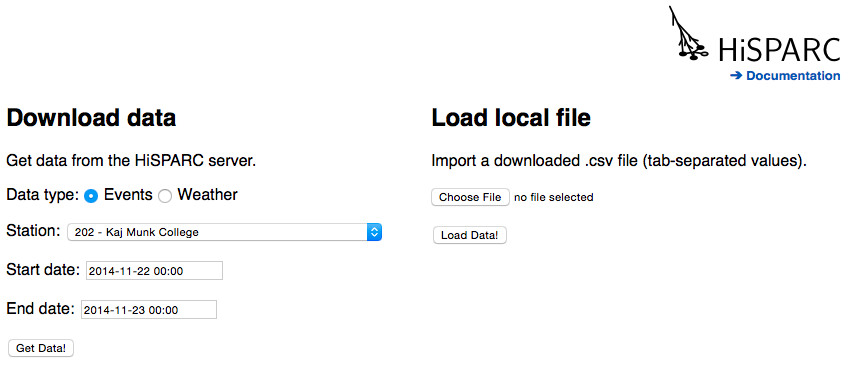
\includegraphics[scale=\screenscale]{tool-landing}
  \caption{Openingspagina van de data retrieval tool.}
  \label{fig:tool-landing}
\end{figure}

\uplevel{In dit werkblad richten we ons op de linkerkolom: \emph{download
data}. Hier is het mogelijk om data van de \hisparc servers te downloaden
in de browser om vervolgens de data te analyseren.}

\question We gaan in eerste instantie \emph{events} downloaden.  Kies
station 501 (Nikhef) en een startdatum van 1 november 2014, en een
einddatum van 2 november 2014. Klik op \emph{Get Data!}.

\uplevel{Tijdens het downloaden wordt het \hisparc logo rechtsbovenaan de
pagina geanimeerd.  De animatie bootst een shower na die op het
aardoppervlak wordt gedetecteerd. Als de animatie stopt is de dataset
gedownload.}

\question Bekijk \figref{fig:tool-dataset}. Dit kopje verschijnt op de
pagina zodra een dataset beschikbaar is. Download voor hetzelfde station
en dezelfde data ook eens meteorologische gegevens (\emph{data type:
weather}).  Download ook eens events voor station 202. Het kopje datasets
komt nu overeen met \figref{fig:tool-datasets}.

\begin{figure}
  \centering
  
\includegraphics[scale=\screenscale]{tool-dataset}
  \caption{Na downloaden is er een dataset beschikbaar.}
  \label{fig:tool-dataset}
\end{figure}

\begin{figure}
  \centering
  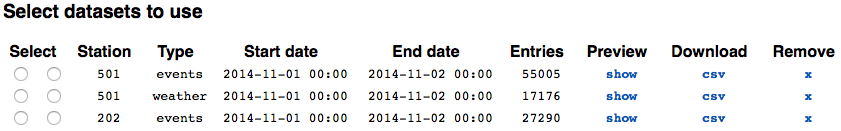
\includegraphics[scale=\screenscale]{tool-datasets}
  \caption{Meerdere datasets kunnen na elkaar worden gedownload.}
  \label{fig:tool-datasets}
\end{figure}

\uplevel{Bekijk \figref{fig:tool-datasets}.  Het getal onder
\emph{entries} is het aantal metingen (events of meteorologische gegevens)
dat beschikbaar is.  Als je klikt op \emph{csv} onder \emph{download}, dan
download je alle data als tekstbestand. Je kunt de gegevens dan inladen in
een ander programma. Om een dataset uit het geheugen te verwijderen klik
je op het kruisje onder \emph{remove}.}

\uplevel{Een overzicht van de ruwe data is beschikbaar door te klikken op
\emph{show} onder \emph{preview}.}

\question Bekijk een preview van de events van station 501. Klik voor het
bovenste event op \emph{show} onder het kopje \emph{trace} helemaal
rechts. Je scherm moet nu overeen komen met
\figref{fig:tool-preview-trace}. De grafiek is een weergave van de ruwe
data van een \hisparc event. Geladen deeltjes zijn door de detectoren
gegaan en hebben een lichtspoor nagelaten. Bekijk de grafiek en bestudeer
de getallen van het eerste event in de tabel. Verklaar de getallen onder
\emph{pulseheights}, \emph{arrival time} en \emph{trigger time}.

\begin{figure}
  \centering
  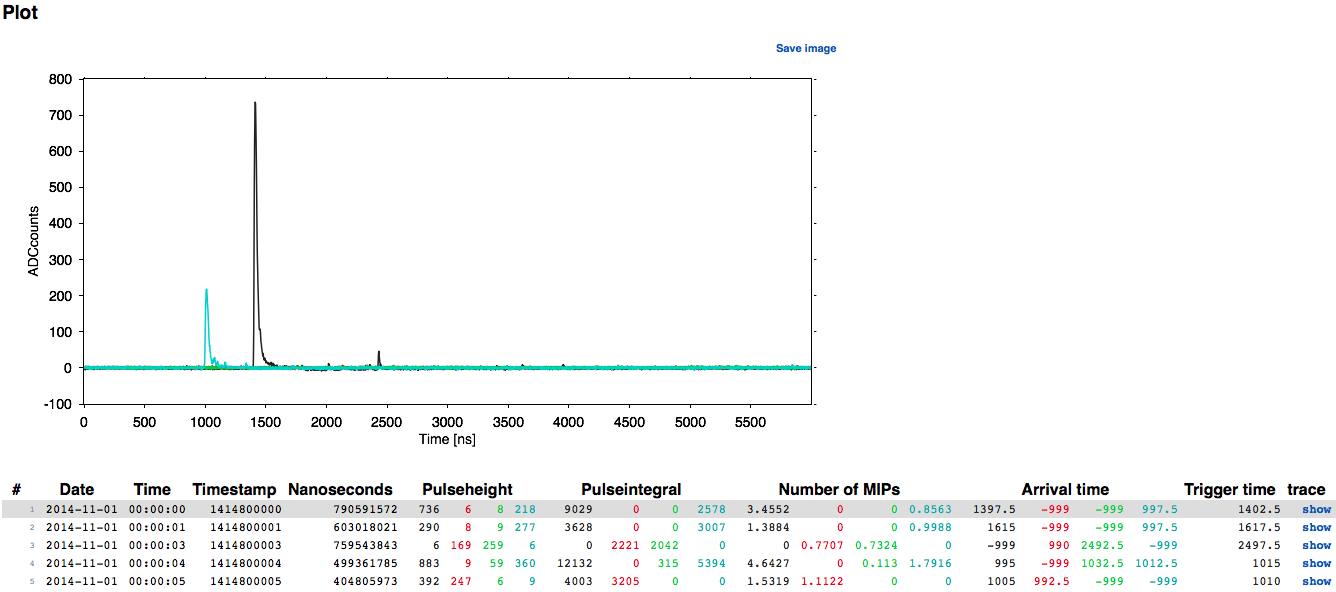
\includegraphics[width=\linewidth]{tool-preview-trace}
  \caption{Preview van een \hisparc event.}
  \label{fig:tool-preview-trace}
\end{figure}

\uplevel{De kolom \emph{pulseintegral} geeft aan hoe groot de oppervlakte
is onder het signaal. Dit is een maat voor hoeveel energie de deeltjes
hebben achtergelaten in de detector en wordt gebruikt om een schatting te
maken van het aantal geladen deeltjes dat door een detector ging. Deze
schatting is weergegeven onder het kopje \emph{number of MIPs}. MIP staat
voor \emph{minimum-ionizing particle}, ofwel een deeltje dat een minimale
hoeveelheid energie verliest door ionisatie. Deeltjes in showers vallen in
deze categorie.}

\uplevel{In de tabel komt soms het getal -999 voor. Dit betekent dat het
niet mogelijk was een voorlopige analyse uit te voeren op de data.  In de
praktijk betekent dit dat er in die detector geen deeltjes zijn
gedetecteerd. Ook kan het getal -1 voorkomen. Dat betekent dat er voor die
kolom geen data beschikbaar is, bijvoorbeeld als je data bekijkt van een
station met twee detectoren, in plaats van vier.}

\question Bekijk een preview van de data van station 202. Hoeveel
detectoren heeft dit station?


\uplevel{\section{Analyse van \hisparc events}}

\uplevel{Om een dataset te analyseren moeten we die eerst selecteren.}

\question Klik op het eerste bolletje van de dataset van events van
station 501. Op de pagina verschijnt nu een stuk met instellingen om een
grafiek te maken (\figref{fig:tool-plot-settings}).

\begin{figure}
  \centering
  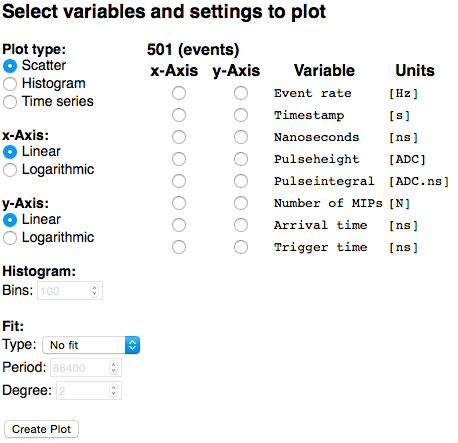
\includegraphics[scale=\screenscale]{tool-plot-settings}
  \caption{Instellingen voor grafieken. Hier kun je kiezen welke gegevens
    je wilt weergeven en wat voor type grafiek je wilt krijgen.}
  \label{fig:tool-plot-settings}
\end{figure}


\uplevel{\subsection{Scatter plots}}

\uplevel{Standaard maak je een \emph{scatter plot}. Dit soort grafieken
maak je ook tijdens een practicum natuurkunde. Je vergelijkt twee gegevens
(bijvoorbeeld kracht en uitrekking van een veer) en voor iedere meting zet
je een punt in de grafiek. Het enige verschil met een `gewoon' practicum
is dat de \hisparc dataset veel meer metingen bevat. In plaats van een
paar punten met een lijn zul je nu vaak een wolk van punten zien.}

\uplevel{Een scatter plot is ideaal om te onderzoeken of bepaalde
grootheden van elkaar afhankelijk zijn (zoals kracht en uitrekking bij een
veer). Als er een verband is, dan zie je dat in de grafiek. Is er
\emph{geen} verband, dan zie je slechts een wolk van punten.}

\question Kies \emph{timestamp} voor de x-as en óók \emph{timestamp} voor
de y-as. Klik dan op \emph{create plot} om een grafiek te maken.

\uplevel{Als variabelen van elkaar afhankelijk zijn, zeggen we ook wel dat
ze met elkaar \emph{correleren}. De grafiek die je net gemaakt hebt is een
extreem voorbeeld. De waardes op de x- en y-as zijn \emph{exact} gelijk.
Je kunt veel leren door correlaties te onderzoeken en te kijken naar de
vorm die verschijnt in de grafieken. Als je nadenkt over \emph{waarom} een
correlatie een bepaalde vorm heeft, kan het helpen om de grafiek nog een
keer te plotten, maar dan de variabelen voor de x- en y-as om te draaien.}

\question Kies \emph{timestamp} voor de x-as en \emph{nanoseconds} voor
de y-as. Klik dan op \emph{create plot} om een grafiek te maken.

\uplevel{Dit is een extreem voorbeeld van \emph{ongecorreleerde}
variabelen. Er is geen samenhang. Dit komt omdat het tijdstip van een
event op een dag (timestamp) niets te maken heeft met of het event aan het
begin van een seconde, middenin een seconde, of aan het eind van een
seconde wordt gemeten (nanoseconds).}

\question Maak een scatter plot met pulshoogte op de x-as, en
pulsintegraal op de y-as. Probeer de vorm te verklaren.

\question Draai het nu om: zet pulsintegraal op de x-as, en pulshoogte op
de y-as. Probeer weer de vorm te verklaren. Zie het antwoord\footnote{In
deze grafiek zie je dat events met een grote integraal (pulsoppervlak),
ook een grote hoogte hebben. In eerste instantie gaat dat gelijk op: als
er meer deeltjes door een detector gaan dan wordt de puls hoger én breder.
Maar als er heel veel deeltjes door een detector gaan, wordt de
oppervlakte van de puls wel (flink) groter, maar niet heel veel meer
hoger. De verklaring hiervoor is dat de elektronica pulsen met een grote
spanning (de `hoogte' van de puls) niet goed aankan.} in de voetnoot. Vind
je dit duidelijker?

\question Onderzoek andere correlaties. Welke grootheid wordt
\emph{direct} gebruikt om een schatting te maken van het aantal MIPs in
een detector?


\uplevel{\subsection{Histogram}}

\uplevel{Een \emph{histogram} is een grafiek waarin wordt aangegeven
\emph{hoe vaak} een bepaalde waarde voorkomt. Bijvoorbeeld: hoeveel
leerlingen hebben een lengte tussen de \SI{1,80}{\meter} en
\SI{1,85}{\meter}?}

\uplevel{Als je als plottype \emph{histogram} kiest, kun je geen y-as meer
kiezen. De grafieken die gemaakt worden hebben een y-as die loopt van de
kleinste tot de grootste waarde.  \emph{Hij begint vaak niet bij nul!}}

\question Maak een histogram van de event rate (het aantal events per
seconde).  Welke event rate komt het meest voor? Hoe groot is de
spreiding?

\question Maak een histogram van de timestamps (tijdstippen van de
events). Als je één dag data hebt, zet het aantal bins dan op 24. In het
histogram verschijnt dan het aantal events per uur.

\question Maak een histogram van de pulshoogten. Maak histogrammen voor
10, 50, 100, 500 en 1000 bins. Wat is het voordeel van veel bins? En wat
is een nadeel?

\uplevel{Als er een groot verschil is tussen bins met veel counts en bins
met weinig counts is het vaak moeilijk om te zien hoe de grafiek precies
loopt. Je kunt dan kiezen voor een \emph{logaritmische} schaalverdeling.}

\question Gebruik een logaritmische y-as in een pulshoogtehistogram met
1000 bins. Geef een verklaring voor de bult in de grafiek.


\uplevel{\subsection{Time series}}

\uplevel{Een \emph{time series} grafiek is een scatter plot waarbij de
tijd langs de x-as staat.  Eigenlijk krijg je precies hetzelfde als je in
een scatter plot kiest voor \emph{timestamps} langs de x-as. Het enige
verschil is dat de tijdstempels worden omgeschreven naar een leesbare
weergave van datum/tijd.}


\uplevel{\subsection{Correlaties met weerdata}}

\uplevel{Bovenaan de pagina, onder het kopje \emph{select datasets to
use}, selecteer de weerdata als tweede dataset. Onder het kopje
\emph{select} staat dan in de eerste kolom een bolletje bij \emph{events},
en in de tweede kolom een bolletje bij \emph{weather}.}

\uplevel{Je kunt nu vrij kiezen uit variabelen van events en weerdata om
met elkaar te plotten. Om een verband (correlatie) tussen twee grootheden
te onderzoeken gebruik je een scatter plot.}

\question Onderzoek een mogelijk verband tussen de luchtdruk en de
temperatuur.

\question Onderzoek een mogelijk verband tussen de luchtdruk en het aantal
gedetecteerde showers per seconde.

\uplevel{Als je denkt een verband gevonden te hebben, kun je bij de
grafiekopties onder het kopje \emph{fit} de computer laten zoeken naar het
precieze verband. Kies eens voor \emph{linear} en maak een nieuwe grafiek.
Onderaan de grafiek staat dan de functie van de beste lijn door de data.
Beoordeel zelf in de grafiek of je vindt dat de computer een goed verband
heeft gevonden. Vaak wordt een verband pas duidelijk als je veel data hebt
verzameld. Eén dag is vaak niet genoeg. Kies dan liever een week of een
maand.}

\question Onderzoek nogmaals het verband tussen luchtdruk en event rate,
en fit een lineaire functie. Zie je een duidelijk verband?


\uplevel{\section{Kort eigen onderzoek}}

\begin{savenotes}
\uplevel{Voor dit eigen onderzoek kun je zelf data downloaden. Je mag zelf
kiezen welke stations je gebruikt,\footnote{Zie ook de kaart op de
\hisparc website: \url{http://data.hisparc.nl/show/stations_on_map/}. Als
je ver inzoomed kun je de stationsnummers zien.} en hoeveel data je nodig
hebt (een dag, een week, een maand, ...). Je kunt denken aan één van
onderstaande opdrachten, maar je mag ook zelf iets verzinnen.}
\end{savenotes}

\question Onderzoek het verband tussen verschillende weergegevens:
luchtdruk en temperatuur, temperatuur en hoeveelheid zonnestraling,
windkracht en windrichting, enz.

\question Onderzoek het verband tussen het aantal waargenomen showers en
weergegevens als luchtdruk, temperatuur, enz.

\question Onderzoek een mogelijke periodiciteit in aantallen waargenomen
showers: zie je bijvoorbeeld overdag meer showers dan 's nachts?

\question Google naar \emph{space weather} o.i.d. en onderzoek of je meer
of minder showers ziet als er zonneuitbarstingen zijn.

\question Ga op zoek naar dagen met onweer (buienradar?). Bekijk de
\hisparc data voor verschillende stations, op het moment dat de
onweersbuien over dreven. Je kunt denken aan aantal events per seconde,
gemiddelde pulsintegraal, maar ook luchtdruk en temperatuur.


\end{questions}
\end{document}
